\section{Аналитика}

\subsection{Описание предметной области}

Геомониторинг автопарка каршеринга - это постоянная система контроля местонахождения автомобилей, которые сдаются в краткосрочную аренду. Каршеринг - это форма использования транспортных средств, при которой клиент получает временный доступ к автомобилю на ограниченный промежуток времени для передвижения по городу. Автопарк каршеринга включает все автомобили, находящиеся в собственности компании и доступные для аренды клиентами. Поскольку такие автомобили эксплуатируются каждый день, перемещаются по большой территории и используются разными водителями, возникает необходимость в непрерывном наблюдении за их местонахождением и техническим состоянием.

Основой геомониторинга является определение местоположения автомобиля в реальном времени. Для этого в каждый автомобиль устанавливается телематический терминал - устройство, предназначенное для сбора и передачи данных. Терминал оснащён спутниковым модулем, который работает одновременно с навигационными системами GPS и ГЛОНАСС, что повышает точность и надёжность определения координат.

GPS - это глобальная спутниковая навигационная система. Она работает так: над Землёй летает группа из 32 спутников на высоте примерно 20 000 километров. Каждый спутник постоянно передаёт радиосигнал, в котором содержится информация о времени отправки сигнала и о том, где именно находится спутник. Приёмник в машине ловит эти сигналы и измеряет, сколько времени сигнал шёл от спутника до приёмника. Зная скорость радиоволн (скорость света), приёмник вычисляет расстояние до каждого спутника. Чтобы точно определить своё положение на Земле, приёмнику нужно поймать сигнал минимум от трех спутников одновременно.

Координаты определяются в системе WGS-84 (World Geodetic System 1984) - это мировой стандарт координат для GPS. В этой системе положение любой точки на Земле описывается тремя числами: широта (насколько далеко от экватора), долгота (насколько далеко от нулевого меридиана) и высота. Система WGS-84 представляет Землю как эллипсоид - немного сплюснутый шар. Центр системы координат WGS-84 совпадает с центром масс Земли, а математические параметры эллипсоида подобраны так чтобы максимально точно описать форму планеты. В городе GPS определяет координаты с точностью 5-15 метров, этого достаточно для каршеринга. В России раньше использовали другие системы координат - СК-42 (система координат 1942 года, Пулково 42) и СК-95 (ПЗ-90, используется в ГЛОНАСС). Но для GPS используется именно WGS-84, потому что это единый стандарт для всего мира, и не нужно пересчитывать координаты при переезде из одной страны в другую.

Чтобы система работала лучше, в телематический терминал встроена ещё одна технология - инерциальная система навигации (ИНС). Это набор датчиков: акселерометры (измеряют ускорение машины) и гироскопы (измеряют повороты). Когда машина заезжает в тоннель или под мост, сигнал со спутников может пропасть. В этот момент инерциальная система продолжает следить за движением машины - она знает последнюю известную точку, скорость и направление, и может примерно посчитать, где машина находится сейчас. Это называется аппроксимация координат - система делает приблизительный расчёт положения на основе данных о движении. Когда сигнал со спутников снова появляется, система GPS корректирует эту погрешность и снова начинает показывать точные координаты. Такая комбинация спутниковой навигации и инерциальных датчиков позволяет непрерывно отслеживать машину даже в сложных городских условиях.

Собранные данные о местоположении автомобиля передаются на сервер компании по сотовым сетям связи 4G (LTE). Для этого в терминале стоит SIM-карта с IoT-тарифом. IoT (Internet of Things) - это когда разные устройства подключены к интернету и автоматически обмениваются данными без участия человека. Например, холодильник может сам заказывать продукты, когда они заканчиваются. В каршеринге телематический терминал - это IoT-устройство: он сам собирает информацию где машина, с какой скоростью едет, сколько топлива осталось и автоматически отправляет эти данные на сервер компании. IoT-тарифы сотовых операторов специально сделаны для таких устройств: они работают круглосуточно, стоят дёшево, работают в любом месте города без разрывов связи и очень надёжные. Данные отправляются либо раз в какое то количество времени, либо когда происходит что-то важное, например машина превысила скорость, резко затормозила, произошёл удар, началась или закончилась аренда.

В случае потери связи по мобильной сети телематический терминал сохраняет данные в свою внутреннюю память обычно от 512 МБ до 2 ГБ. Этого хватает, чтобы сохранить информацию о поездках за несколько дней. Система на сервере компании не паникует сразу, если связь с машиной пропала - она ждёт 5-10 минут, потому что связь может временно пропасть из-за помех или плохого покрытия сети. Если связь не появляется после этого времени, внешняя серверная система автоматически создаёт уведомление и отправляет его операторам. Важный момент: анализ ситуации и решение о том, что нужно действовать, принимает не сама машина, а серверная система компании. Сервер постоянно следит за всеми машинами автопарка, проверяет поступающие данные, сравнивает их с нормальными показателями и создаёт тревожные сообщения для операторов, если что-то идёт не так.

Операторы колл-центра связываются с клиентом, который использует машину, чтобы выяснить, что случилось. Если клиент не отвечает или обнаружена неисправность, на последнее известное место, где была машина, отправляется сервисная бригада. Эти специалисты ищут машину, заправляют её, заряжают или устраняют мелкие поломки.

Системой геомониторинга пользуются различные категории людей. Клиенты каршеринга через мобильное приложение видят автомобили на карте, их координаты и уровень топлива или заряда, что позволяет выбрать подходящую машину. Операторы колл-центра используют систему для контроля текущих поездок, помощи клиентам и обработки нештатных ситуаций. Передвижные сервисные группы получают задания с указанием конкретных автомобилей и их координат для технического обслуживания. Аналитики компании используют данные для анализа загрузки автопарка, выявления зон дефицита или избытка автомобилей и оптимизации распределения машин по городу.

\textbf{Ключевой процесс 1 - построение трека движения автомобиля.} Телематический терминал непрерывно фиксирует координаты автомобиля и отправляет их на сервер с интервалом 10-15 секунд. Серверная система принимает каждую новую точку с координатами, временной меткой и последовательно записывает все полученные точки в базу данных, формируя трек движения. Для каждого автомобиля ведётся отдельный трек, который показывает весь маршрут за определённый период времени. По этим данным система строит линию на карте, соединяющую все точки в хронологическом порядке, что позволяет визуально увидеть, где именно ездила машина. В этом процессе участвуют несколько ролей: клиент каршеринга непосредственно управляет автомобилем во время поездки, а телематический терминал в фоновом режиме собирает координаты и отправляет их на сервер компании, оператор колл-центра в реальном времени наблюдает за движением автомобиля на карте и может отследить текущее местоположение любой машины из автопарка если поступил запрос от клиента или возникла нештатная ситуация, аналитик компании работает с архивными треками за прошедшие периоды и строит отчёты по пробегам, популярным маршрутам и зонам активности, а администратор системы следит за корректностью поступления данных от всех терминалов и настраивает параметры записи треков в базу данных. Трек сохраняется в архиве и используется для анализа: расчёта пробега, определения времени нахождения в конкретных зонах, проверки соблюдения разрешённой территории эксплуатации, расследования инцидентов и споров с клиентами. Результатом процесса является полная история перемещений каждого автомобиля с точной географической привязкой, доступная для просмотра и анализа операторами и аналитиками компании.

\textbf{Ключевой процесс 2 - определение зон парковки и контроль завершения аренды.} Когда клиент завершает аренду через мобильное приложение, серверная система фиксирует финальные координаты автомобиля и начинает анализ местоположения. Программа на сервере проверяет, находится ли автомобиль в пределах разрешённой зоны завершения аренды - это может быть вся территория города или определённые районы в зависимости от тарифа. Дальше система определяет тип места парковки: на улице в зоне бесплатной парковки, на платной парковке, во дворе жилого дома, на территории торгового центра. Для этого сервер сравнивает координаты с заранее загруженными границами парковочных зон. Если автомобиль припаркован в запрещённом месте вне парковочной зоны, сервер отклоняет завершение аренды и уведомляет клиента о необходимости переместить автомобиль в правильное место. В этом процессе ключевую роль играет клиент каршеринга, который паркует автомобиль в конце поездки и через мобильное приложение нажимает кнопку завершения аренды, после чего приложение показывает ему результат проверки координат и либо подтверждает завершение либо просит переставить машину в другое место, оператор колл-центра вмешивается в процесс только если у клиента возникли вопросы по парковке или система зафиксировала нарушение правил, администратор системы заранее загружает в базу данных актуальные границы разрешённых парковочных зон и обновляет их при изменении городских правил парковки, а аналитик компании изучает статистику по местам завершения аренды и выявляет зоны где скапливается слишком много автомобилей или наоборот где машин не хватает чтобы предложить корректировки тарифов или бонусов за парковку в нужных местах. Также система проверяет расстояние от припаркованного автомобиля до других машин автопарка - если в одном месте скапливается слишком много автомобилей, система может предложить клиенту скидку за парковку в дефицитной зоне или наоборот, доплату за парковку в зоне избытка. После успешной проверки система фиксирует координаты парковки, делает запись в базу данных и отображает автомобиль на карте как доступный для следующего клиента. Результатом процесса является корректное размещение автомобиля на парковке в разрешённой зоне с зафиксированными координатами, что обеспечивает равномерное распределение автопарка по городу и соблюдение правил парковки.

\subsection{Цели функционирования базы данных}

\begin{enumerate}
\item Хранение треков движения автомобилей. База данных должна сохранять все координаты автомобилей с временными метками, чтобы система могла строить треки движения.

\item Хранение зон парковки. База данных должна хранить границы зон парковки, чтобы система могла проверять правильность завершения аренды и предлагать клиентам корректные места для парковки.

\item Хранение тревожных событий связанных с автомобилем. База данных должна фиксировать все инциденты, такие как превышение скорости, резкое торможение, удар, попытки угона, чтобы операторы могли оперативно реагировать на нештатные ситуации.

\item Хранение обращений персонала к данным геомониторинга. База данных должна сохранять все запросы операторов, администраторов к данным геомониторинга, чтобы можно было отслеживать кто и когда обращался к информации о местоположении автомобилей и какие данные запрашивал.
\end{enumerate}

\subsection{Сущности предметной области и их атрибуты}

\begin{enumerate}
	\item \textbf{Автомобиль} -- транспортное средство, которым владеет каршеринг.
\begin{itemize}
\item Гос номер -- государственный регистрационный знак автомобиля
\item Марка -- производитель автомобиля(TODO)
\item Модель -- название модели автомобиля
\item Год выпуска -- год производства автомобиля
\item VIN-номер -- уникальный идентификационный номер транспортного средства
\item Текущий статус -- состояние автомобиля (свободен, в аренде, на обслуживании, неисправен)
\end{itemize}

\item \textbf{Трек движения} -- траектория перемещения автомобиля внутри одной поездки.
\begin{itemize}
\item Время начала трека -- момент начала записи маршрута движения
\item Время окончания трека -- момент завершения записи маршрута движения
\item Статус трека -- состояние записи (активный, завершён, архивный)
\item Вид трека -- категория маршрута (пользовательский, сервисный)
\end{itemize}

\item \textbf{Координаты точки трека} -- географическая точка с временной меткой на маршруте автомобиля.
\begin{itemize}
\item Широта -- географическая широта в системе координат WGS-84
\item Долгота -- географическая долгота в системе координат WGS-84
\item Скорость движения -- скорость автомобиля в момент измерения в км/ч
\item Источник данных -- система определения координат (GPS, инерциальная система)
\end{itemize}

\item \textbf{Зона парковки} -- территория для завершения аренды и парковки автомобилей.
\begin{itemize}
\item Название -- наименование зоны парковки
\item Тип зоны -- категория парковки (бесплатная, платная, запрещённая)
\item Район города -- административный район расположения зоны
\item Максимальное количество автомобилей -- лимит машин которые могут одновременно находиться в зоне
\item Статус активности зоны -- признак доступности зоны для использования
\end{itemize}

\item \textbf{Координаты зоны парковки} -- вершины полигона определяющего границы зоны парковки на карте.
\begin{itemize}
\item Номер вершины по порядку -- порядковый номер точки в контуре полигона
\item Широта -- географическая широта вершины в системе координат WGS-84
\item Долгота -- географическая долгота вершины в системе координат WGS-84
\end{itemize}

\item \textbf{Тревожное событие} -- инцидент или нештатная ситуация зафиксированная системой мониторинга автомобиля.
\begin{itemize}
\item Тип события -- категория инцидента (потеря связи, превышение скорости, резкое торможение, удар, попытка угона, выезд за границу)
\item Широта -- географическая широта места события
\item Долгота -- географическая долгота места события
\item Описание события -- текстовая информация о произошедшем инциденте
\item Статус обработки -- состояние реагирования на событие (новое, в работе, закрыто)
\end{itemize}

\item \textbf{Сотрудник} -- работник компании имеющий доступ к системе геомониторинга автопарка.
\begin{itemize}
\item ФИО -- полное имя сотрудника (фамилия, имя, отчество)
\item Логин -- учётная запись для входа в систему
\item Статус -- текущее состояние сотрудника (активен, в отпуске, уволен, заблокирован)
\item Должность -- занимаемая позиция в компании
\end{itemize}

\item \textbf{Тип сотрудника} -- категория работника определяющая его роль и права доступа.
\begin{itemize}
\item Название типа -- наименование категории (оператор колл-центра, администратор системы, сервисный специалист, аналитик)
\item Описание -- текстовое пояснение роли и функций данного типа сотрудника
\end{itemize}

\item \textbf{Обращения к геомониторингу} -- обращение сотрудника к системе для получения данных о местоположении.
\begin{itemize}
\item Тип запроса -- категория запрашиваемых данных (текущие координаты, история событий)
\item Цель запроса -- причина обращения к данным о местоположении автомобиля
\end{itemize}
\end{enumerate}

\subsection{Перечень ролей}
\begin{enumerate}
\item \textbf{Клиент каршеринга} - человек, который арендует автомобиль. В приложении он может найти машину на карте, начать поездку и потом её закончить.
\item \textbf{Оператор колл-центра} - сотрудник, который следит за всеми машинами на карте, помогает клиентам с вопросами по аренде и реагирует на нештатные ситуации.
\item \textbf{Сервисная бригада} - специалисты, которые выполняют техническое обслуживание, перегонку автомобилей. Они получают задания от системы, которая указывает конкретные машины и их координаты для обслуживания, заправки или ремонта.
\item \textbf{Администратор системы} - человек, который отвечает за настройку и поддержку системы геомониторинга. Он загружает данные о зонах парковки, следит за корректностью поступления данных от терминалов и управляет правами доступа сотрудников.
\end{enumerate}	
\newpage
\clearpage
\newgeometry{paperwidth=420mm,paperheight=297mm,margin=-2mm}

\begin{landscape}
  \thispagestyle{empty}
  \captionsetup{font=small,skip=4pt}

  \begin{figure}[!p]
    \centering
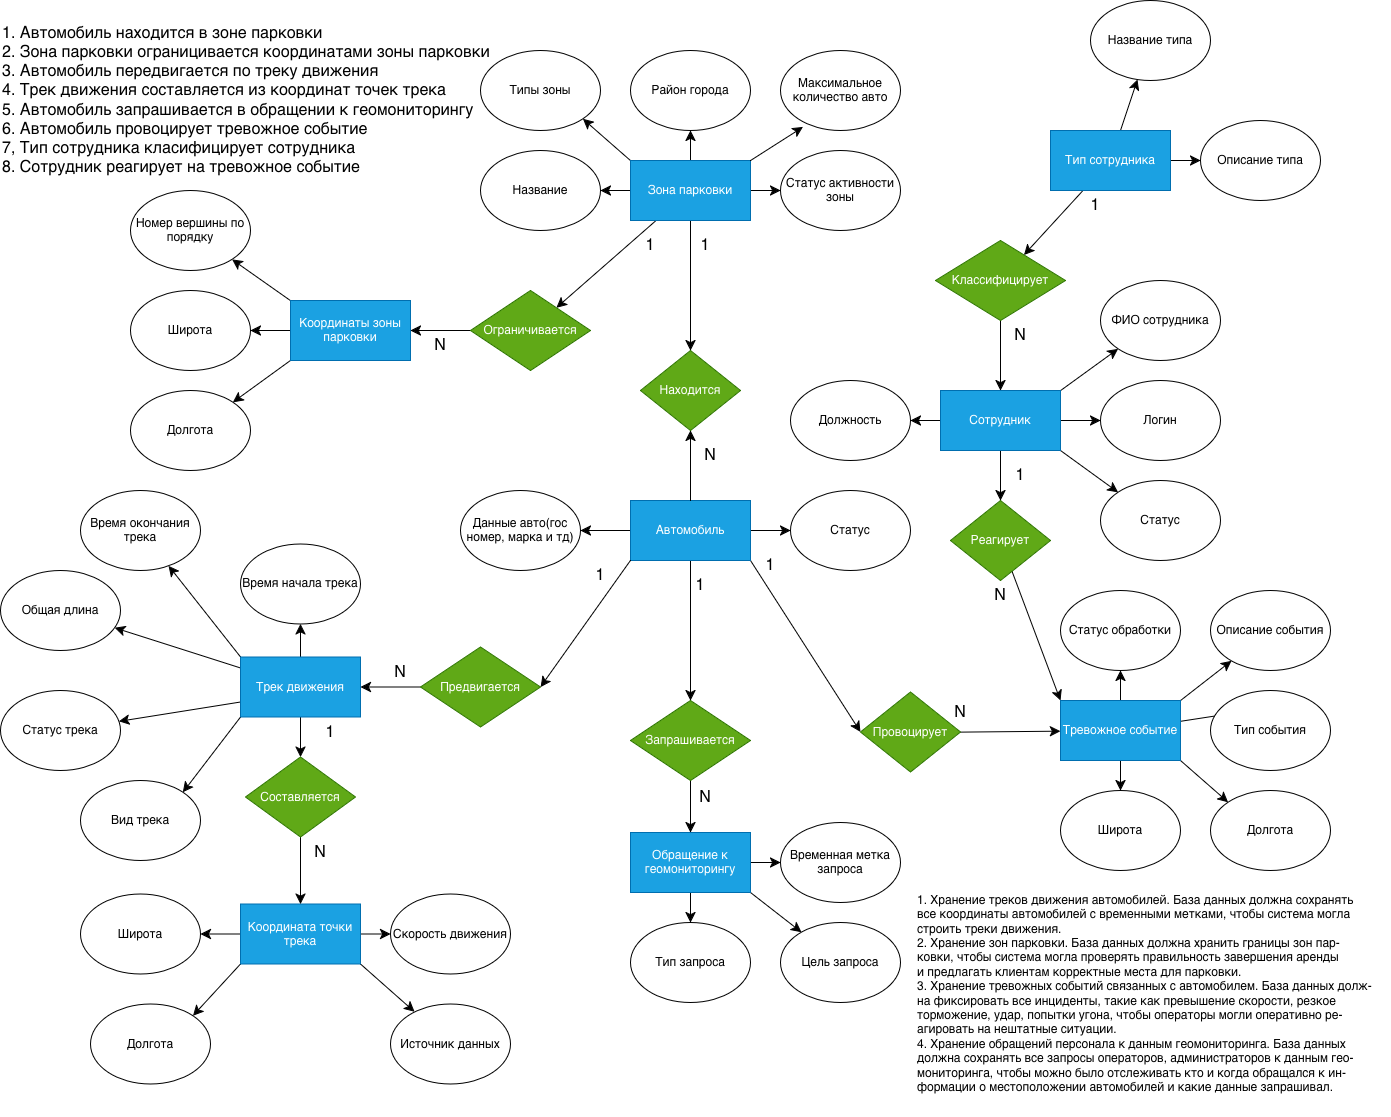
\includegraphics[width=\linewidth,height=\dimexpr\textheight-4\baselineskip\relax,keepaspectratio]{myPhoto/er-diag.png}
    \caption{ER--диаграмма}
    \label{fig:placeholder}
  \end{figure}
\end{landscape}

\restoregeometry
\clearpage

\newpage
\subsection{Схема связи обьектов предметной области}

\begin{figure}[h!]
\centering
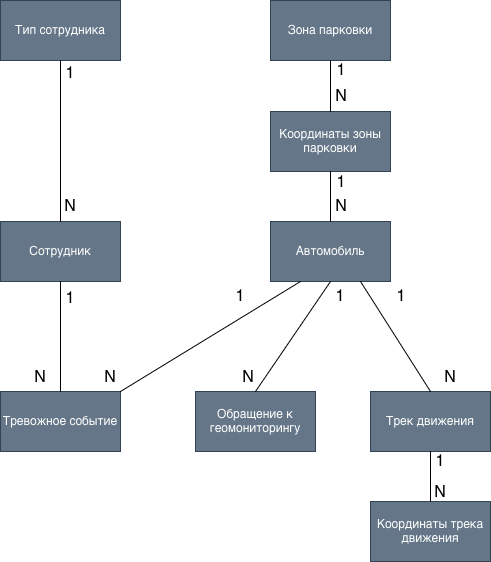
\includegraphics[width=0.6\textwidth]{myPhoto/schema.png}
\caption{Схема связи обьектов предметной области}
\end{figure}